
\documentclass{article}
\usepackage[margin=1in]{geometry}
\usepackage{xcolor}
\usepackage{amsmath}
\usepackage{booktabs}
\usepackage{graphicx}

\title{CSE 318 - Assignment 3}
\author{Anik Saha - 2005001}

\begin{document}
\maketitle

This report summarizes the results of running various constructive and perturbative heuristics on the Traveling Salesman Problem (TSP) for the \textbf{a280.tsp, berlin52.tsp, bier127.tsp, ch130.tsp, ch150.tsp, eil101.tsp, eil51.tsp, eil76.tsp, kroA100.tsp, kroB100.tsp, kroC100.tsp, kroD100.tsp, kroE100.tsp, lin105.tsp, lin318.tsp, pr124.tsp, pr144.tsp, pr76.tsp, rat195.tsp, rat99.tsp, st70.tsp} problem instances.

\section*{Summary Statistics}
\begin{itemize}
  \item Total number of TSP problem files: 21
  \item Total number of constructive heuristics: 6
  \item Total number of perturbative heuristics: 4
\end{itemize}

\section*{Constructive Heuristics}
\begin{itemize}
    \item \textbf{NearestNeighbour}
    \item \textbf{SemiGreedyNearestNeighbour}
    \item \textbf{CheapestInsertion}
    \item \textbf{SemiGreedyCheapestInsertion}
    \item \textbf{SemiGreedyRandomInsertion}
    \item \textbf{MSTSimple}

\end{itemize}

\section*{Perturbative Heuristics}
\begin{itemize}
    \item \textbf{---}
    \item \textbf{TwoOpt}
    \item \textbf{NodeSwap}
    \item \textbf{NodeShift}

\end{itemize}



\newpage
   
\section*{Results}

In the following tables and figures, the relative performances of the constructive and perturbative algorithms are analyzed according to mean values over 10 test runs for each combinations. 

\begin{figure}[h]
\centering
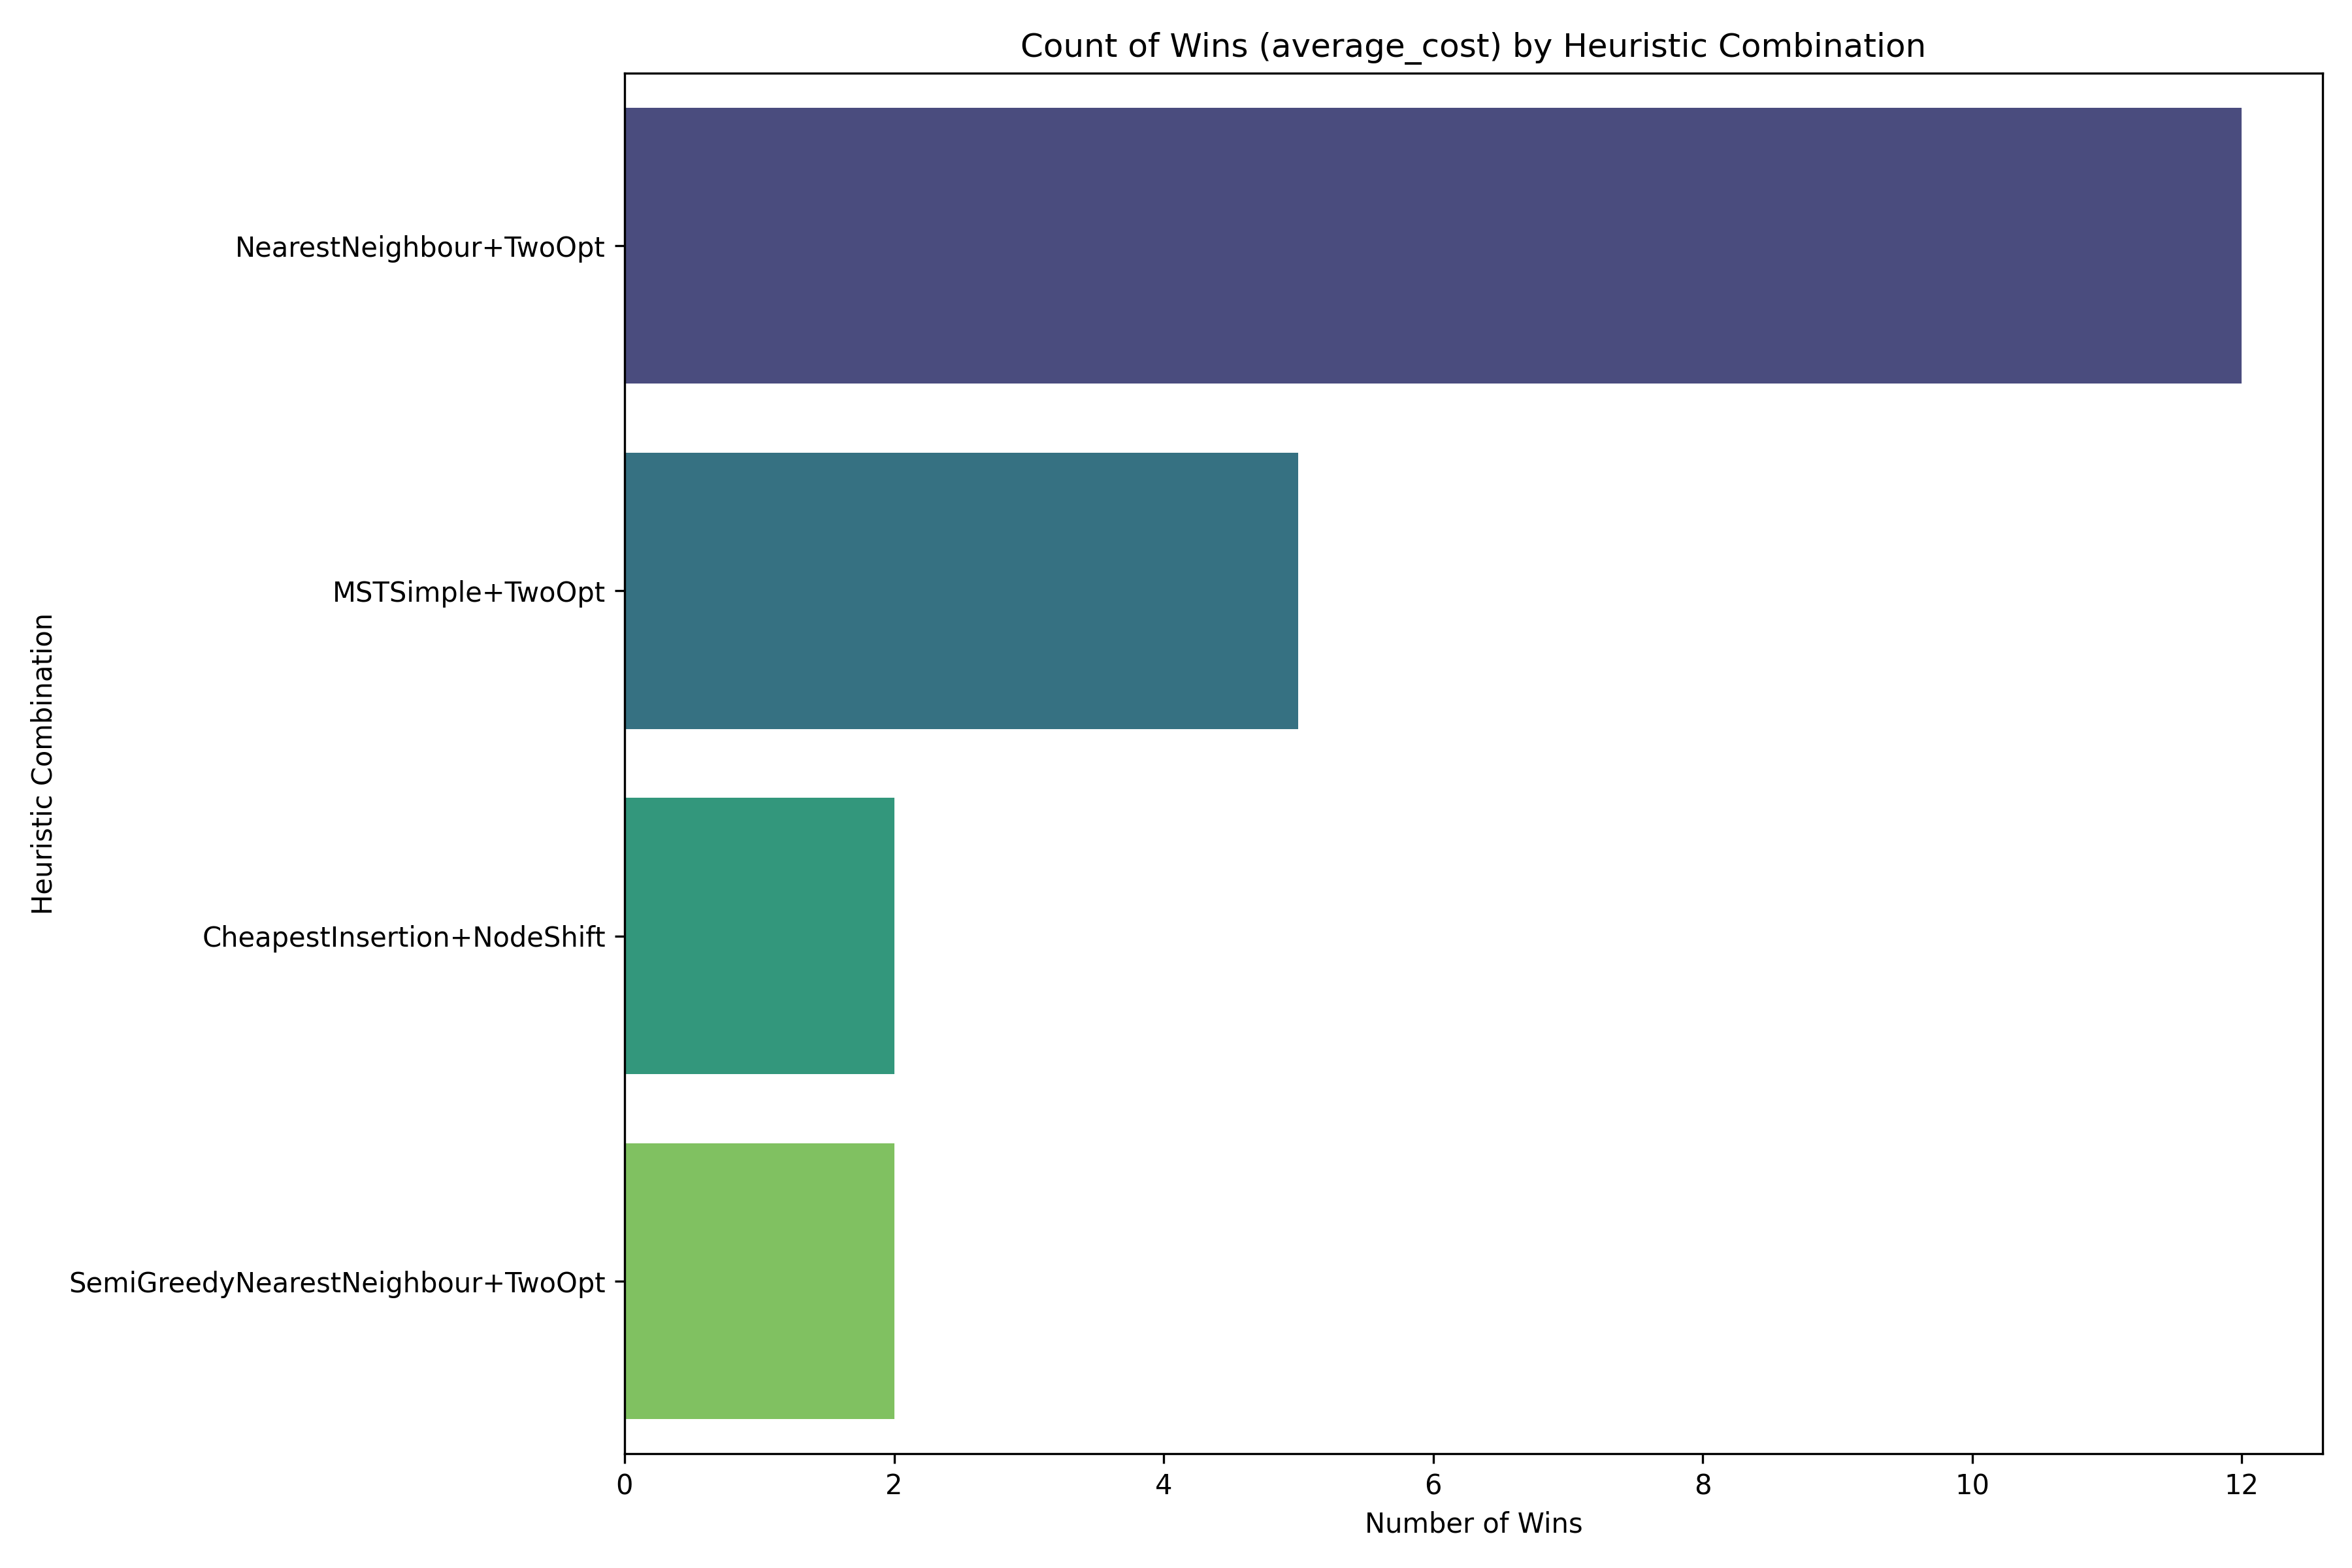
\includegraphics[width=\textwidth]{figures/count-of-wins-comparison.png}
\caption{Count of Wins (average wins) by Heuristic Combination}
\end{figure}


\begin{figure}[h]
\centering
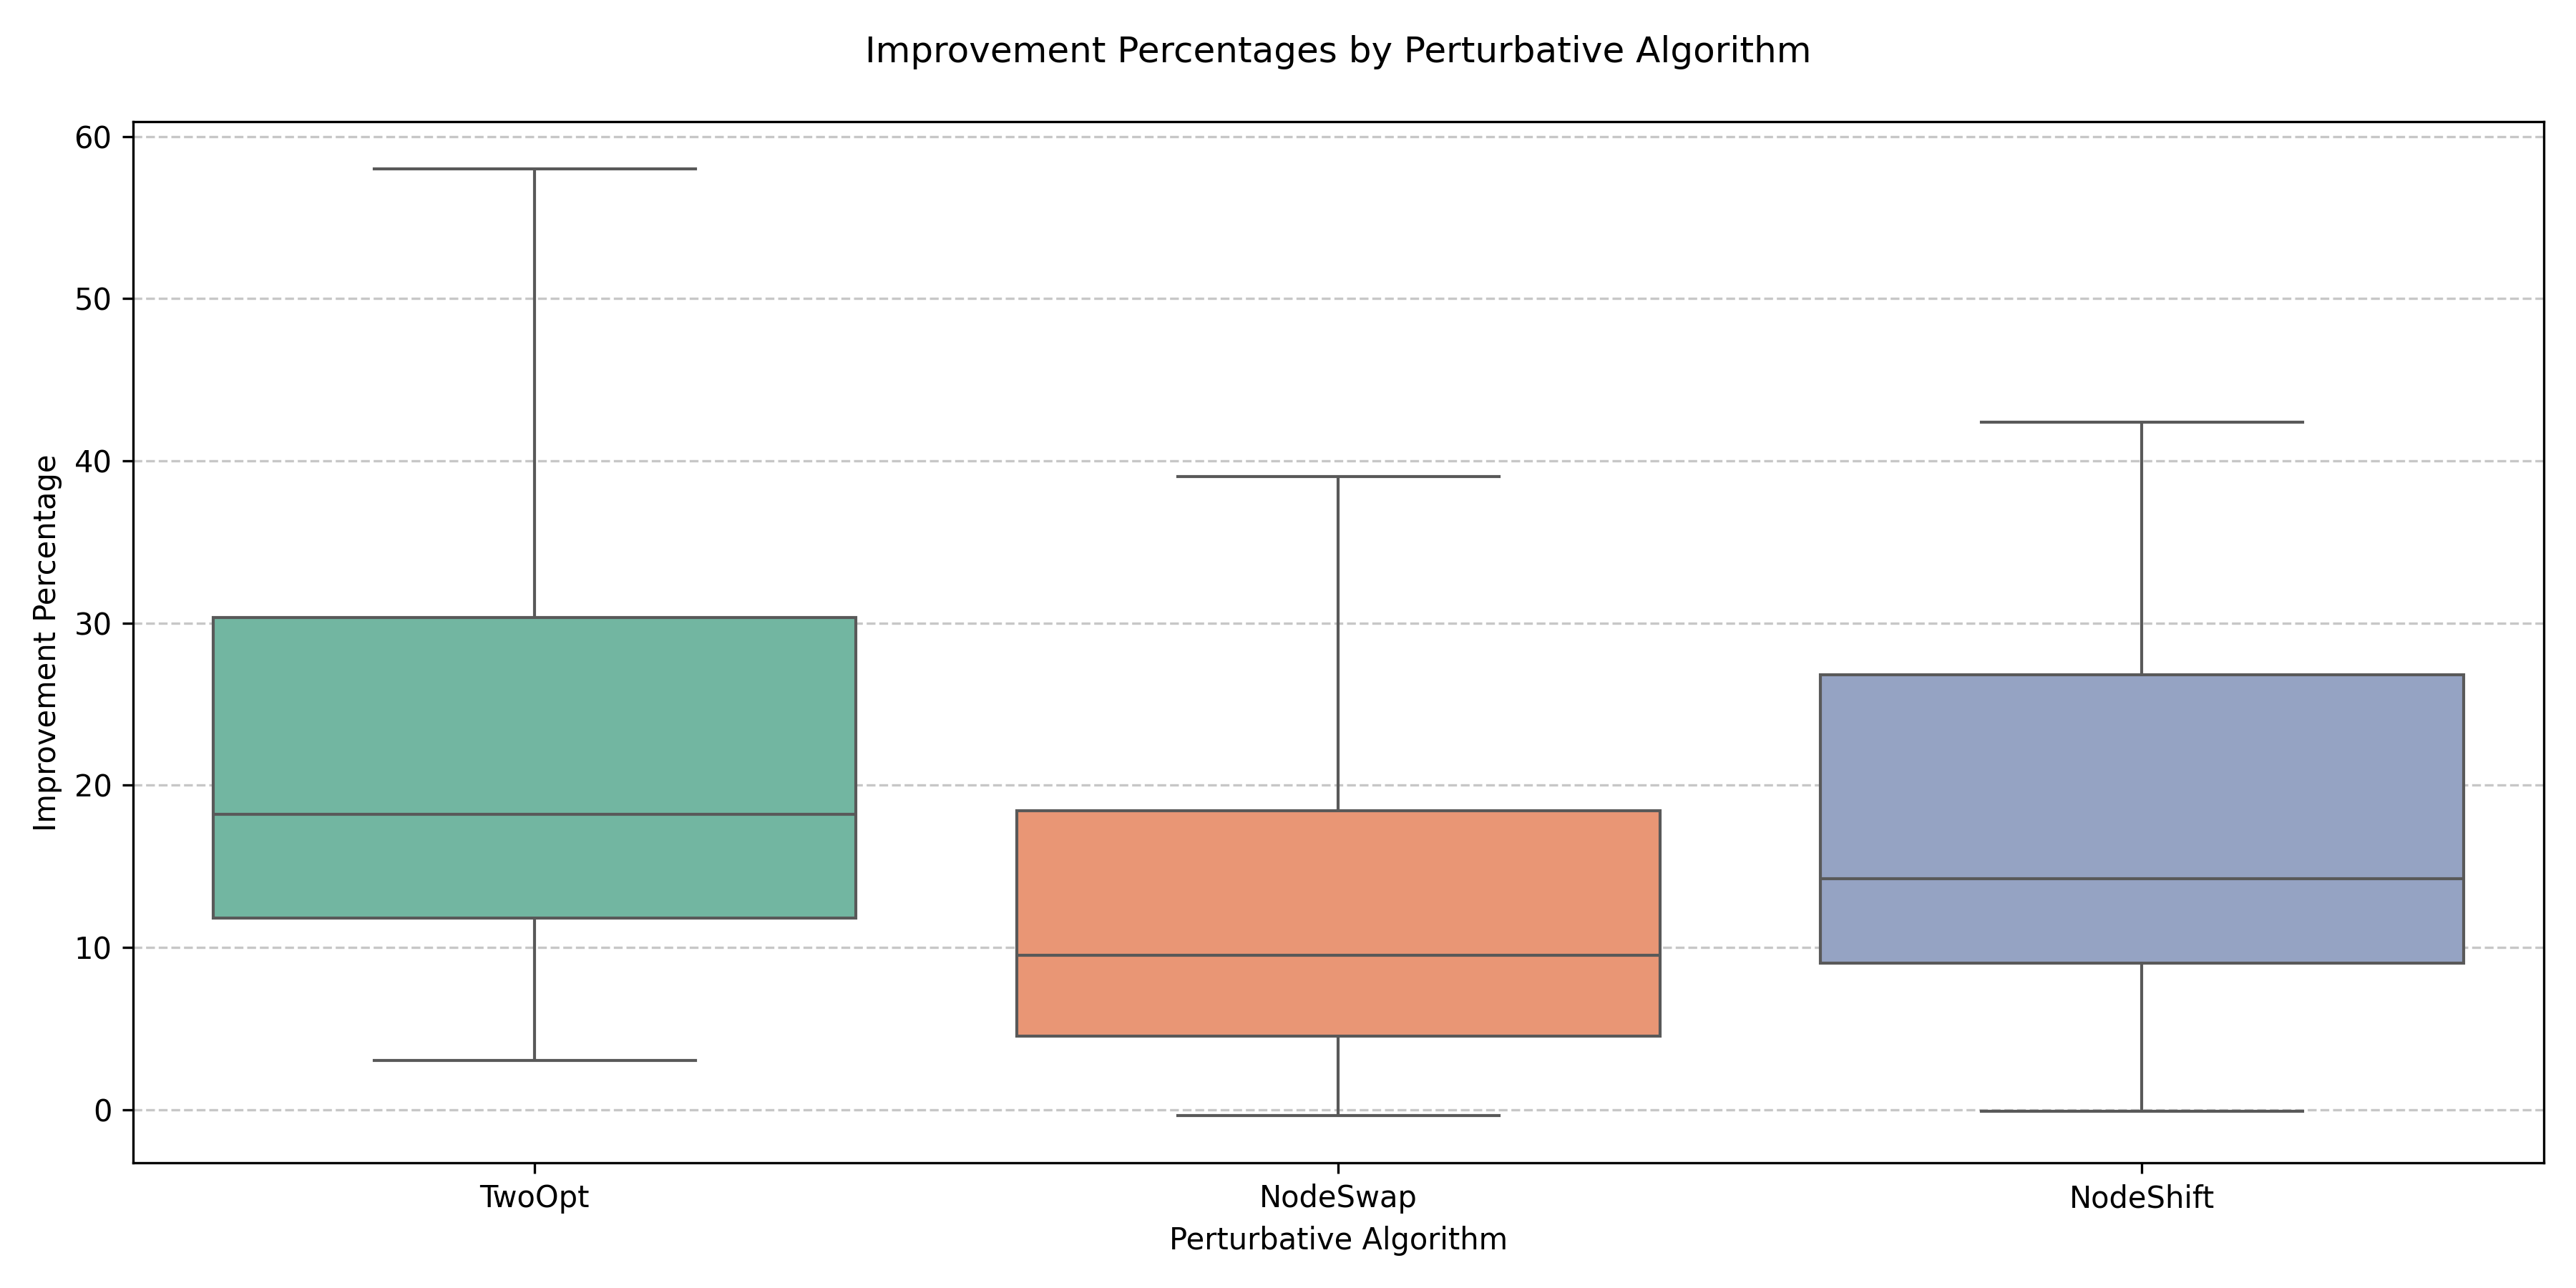
\includegraphics[width=\textwidth]{figures/perturbative-improvement-pct.png}
\caption{Improvement Percentages by Perturbative Algorithm}
\end{figure}



\begin{table}[h]
\centering
\begin{tabular}{llc}
\toprule
Constructive & Perturbative & Mean Deviation \\
\midrule
CheapestInsertion & --- & 0.0465 \\
CheapestInsertion & NodeShift & 0.0432 \\
CheapestInsertion & NodeSwap & 0.0423 \\
CheapestInsertion & TwoOpt & 0.0526 \\
MSTSimple & --- & 0.0447 \\
MSTSimple & NodeShift & 0.0545 \\
MSTSimple & NodeSwap & 0.0583 \\
MSTSimple & TwoOpt & 0.0525 \\
NearestNeighbour & --- & 0.1252 \\
NearestNeighbour & NodeShift & 0.0973 \\
NearestNeighbour & NodeSwap & 0.1246 \\
NearestNeighbour & TwoOpt & 0.0636 \\
SemiGreedyCheapestInsertion & --- & 0.0863 \\
SemiGreedyCheapestInsertion & NodeShift & 0.0756 \\
SemiGreedyCheapestInsertion & NodeSwap & 0.0781 \\
SemiGreedyCheapestInsertion & TwoOpt & 0.0708 \\
SemiGreedyNearestNeighbour & --- & 0.2118 \\
SemiGreedyNearestNeighbour & NodeShift & 0.1495 \\
SemiGreedyNearestNeighbour & NodeSwap & 0.1680 \\
SemiGreedyNearestNeighbour & TwoOpt & 0.0769 \\
SemiGreedyRandomInsertion & --- & 0.0903 \\
SemiGreedyRandomInsertion & NodeShift & 0.1076 \\
SemiGreedyRandomInsertion & NodeSwap & 0.1159 \\
SemiGreedyRandomInsertion & TwoOpt & 0.0749 \\

\bottomrule
\end{tabular}
\caption{Algorithm Combination Consistency Analysis}
\end{table}


\begin{figure}[h]
\centering
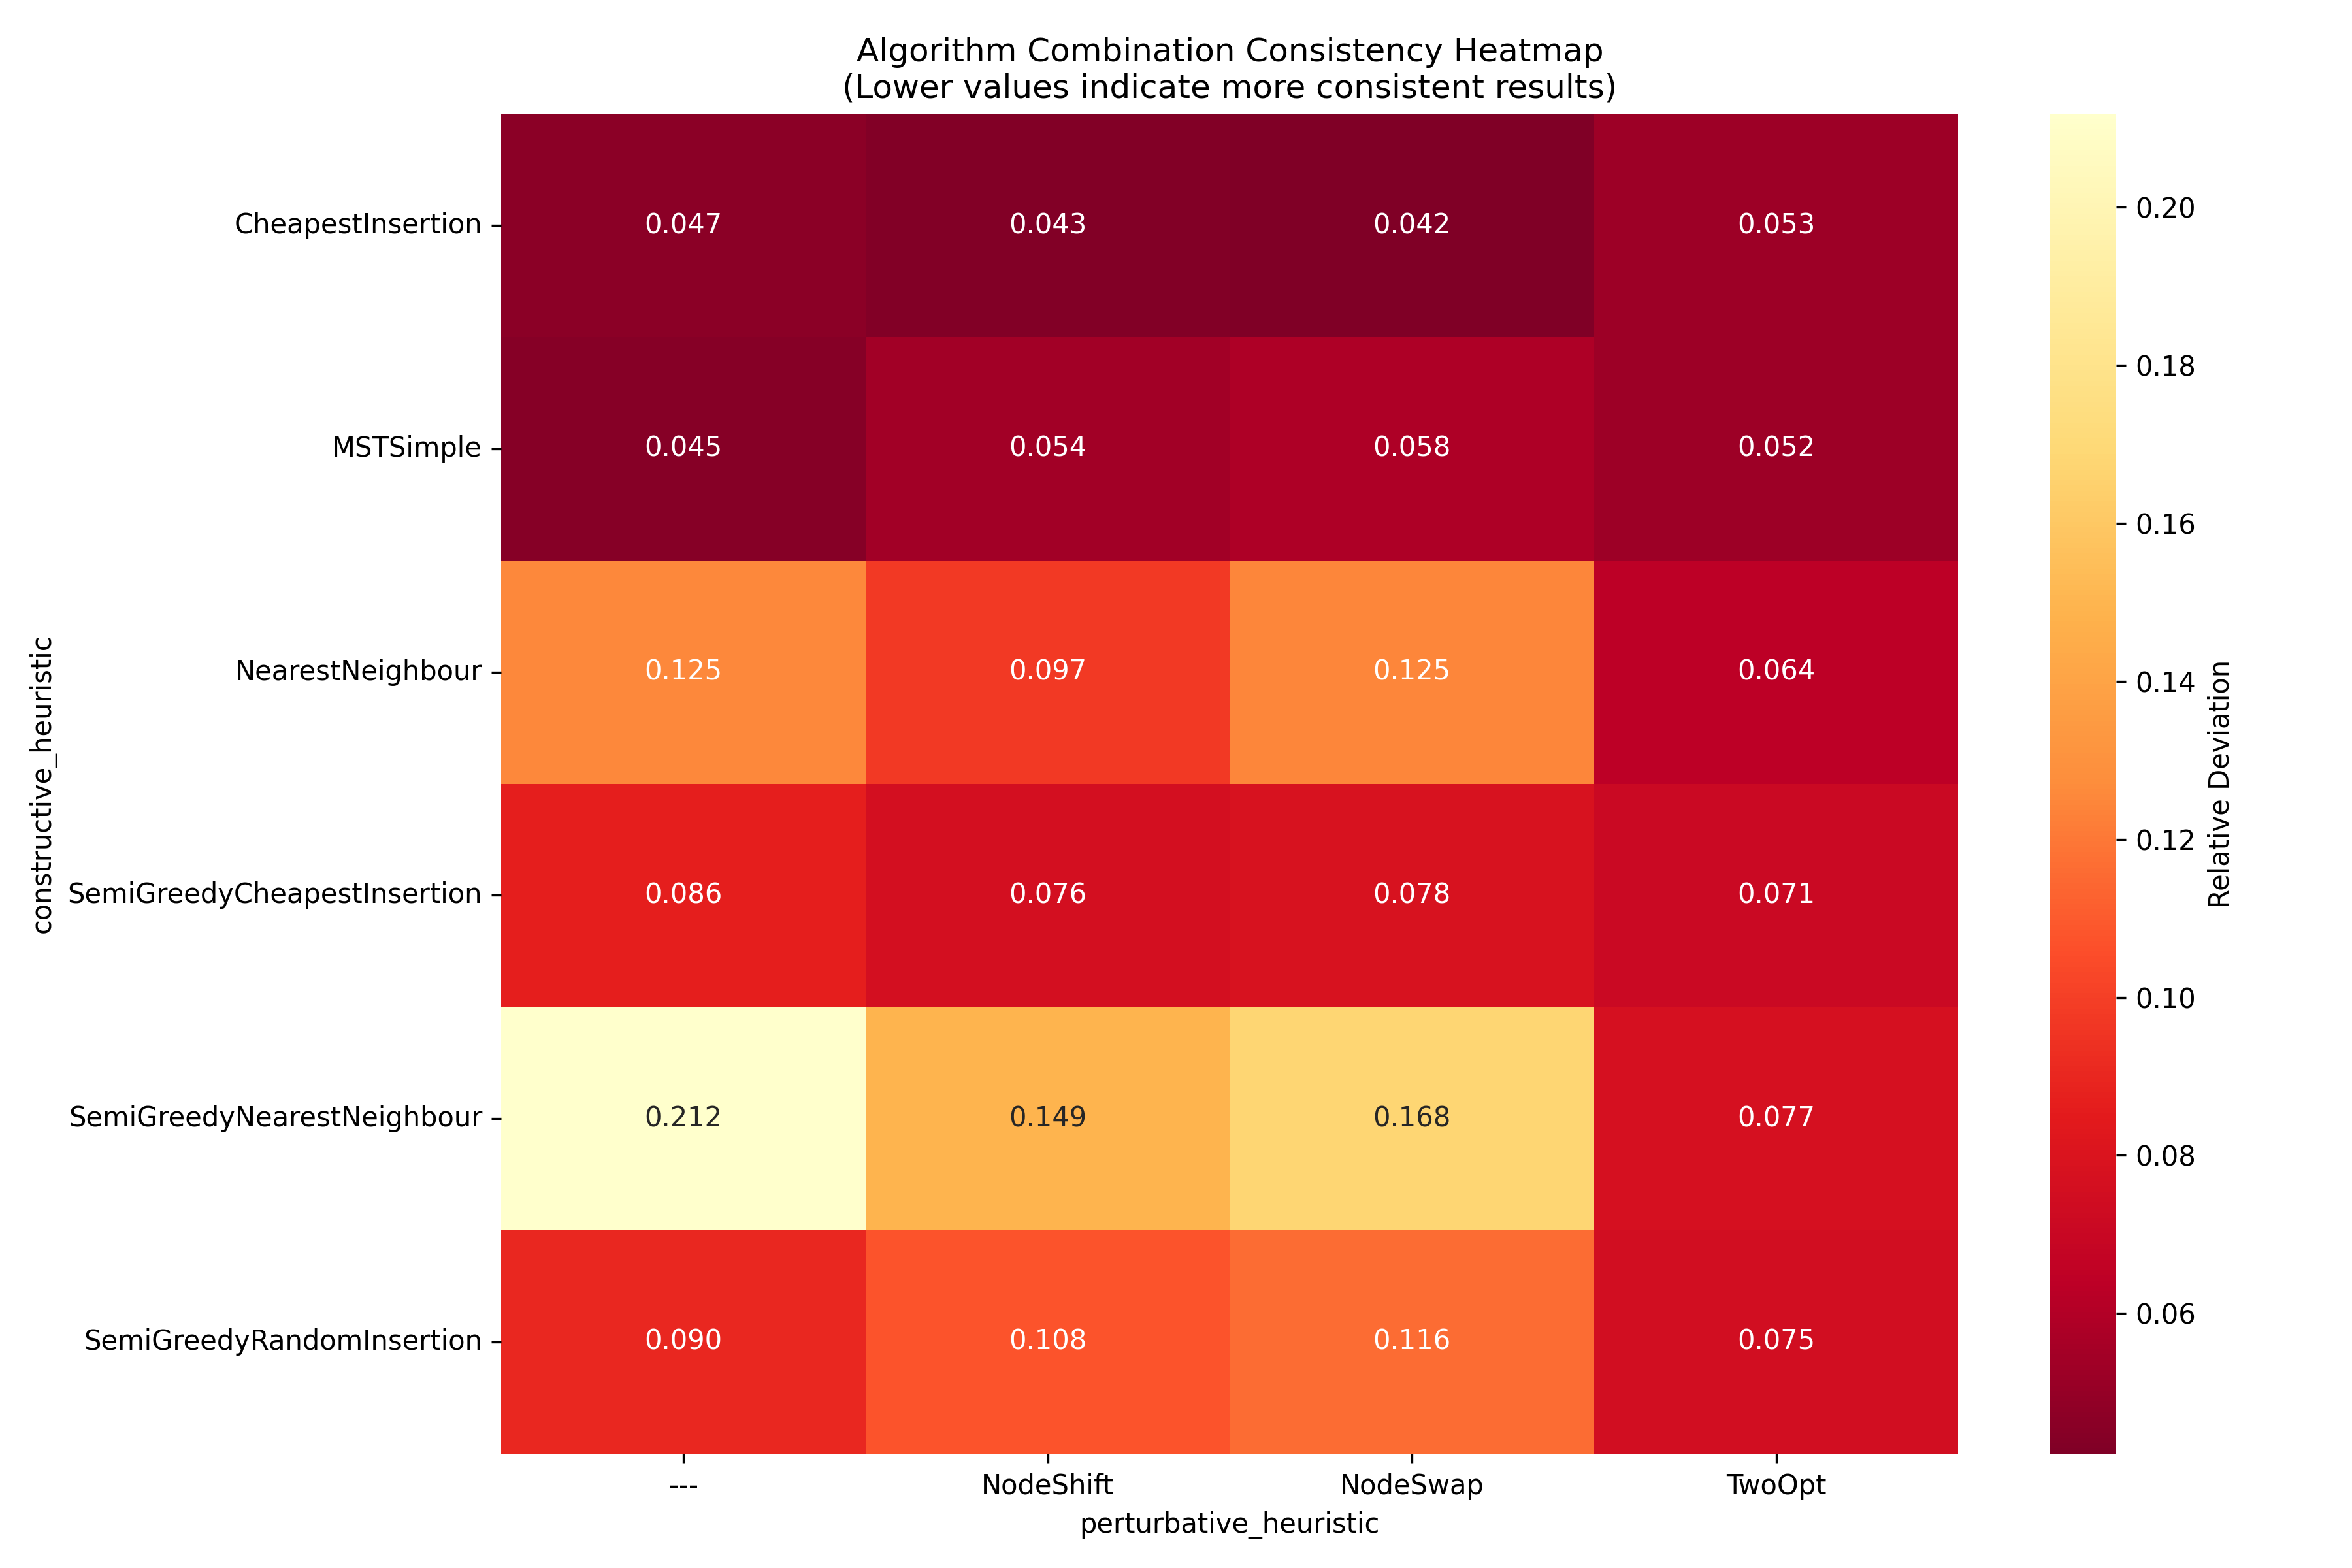
\includegraphics[width=\textwidth]{figures/algo-variation-analysis.png}
\caption{Algorithm Combination Consistency Heatmap (Lower values indicate more consistent results)}
\end{figure}

\end{document}
